% chapters/13/section-01.tex
\section{Menyusun Level}
\label{sec:menyusun-level}

\subsection{Greyboxing}

Level pertama sebaiknya disusun dari balok abu-abu tanpa tekstur, tanpa warna,
dan tanpa aset. Cara itu disebut \istilah{greyboxing}, dan tujuannya bukan
keindahan, melainkan \textbf{menguji mekanik permainannya} sebelum aset yang
mahal dibuat.

Alasannya sederhana: mengubah susunan balok jauh lebih murah daripada mengubah
aset yang sudah dibuat sesuai susunan lama. Apabila ternyata jalur pemainnya
terlalu sempit, atau lompatannya terlalu jauh, yang perlu diubah hanyalah letak
beberapa balok.

Perhatikan Gambar~\ref{fig:editor-fisika}. Level pada gambar itu tersusun dari
balok abu-abu, tangga, dan bongkahan---seluruhnya tanpa tekstur.

\begin{figure}[htbp]
\centering
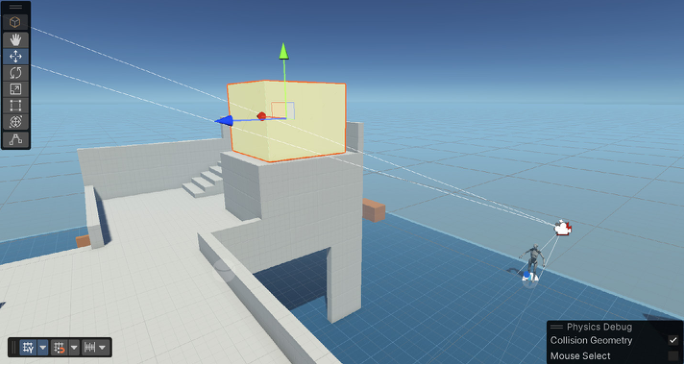
\includegraphics[width=0.9\textwidth]{figures/editor-fisika.png}
\caption{Level yang disusun secara \istilah{greyboxing}, dengan bentuk batas benda ditampilkan pada panel \istilah{Physics Debug}}
\label{fig:editor-fisika}
\sumber{[R12] halaman 66, dengan penyesuaian keterangan}
\end{figure}

Perhatikan pula kotak berwarna kuning pada gambar itu, yaitu bentuk batas
benda yang ditampilkan oleh mesin. Kotak itu menunjukkan batas yang dipakai
untuk memeriksa tabrakan, dan bukan bentuk yang terlihat pemain. Cara
menampilkannya dijelaskan pada Bagian~\ref{sec:masalah-fisika}.

\subsection{Menyusun Level dengan Tilemap}

Selain balok, level dua dimensi dapat disusun dengan \istilah{tilemap}, yaitu
lembaran petak yang dapat diisi dengan pola. Cara itu dipakai untuk level yang
petaknya berulang, misalnya lantai dan dinding.

\istilah{Tilemap} pada Unity tersusun atas dua hal: \istilah{Tilemap} sebagai
lembarannya, dan \istilah{Tilemap Collider 2D} sebagai bentuk batasnya.
Keuntungannya, seluruh petak yang tersusun itu hanya memerlukan satu
\istilah{Collider}, sehingga jauh lebih ringan daripada susunan balok yang
sama banyaknya.

\subsection{Mengukur Ukuran Level}

Ukuran seluruh unsur level sebaiknya ditetapkan lebih dahulu, sebagaimana
dijelaskan pada Bagian~2.3 tentang \istilah{metrics}. Pada Unity, satuan
dasarnya adalah meter, sehingga angka itu langsung bermakna.

Tiga ukuran yang perlu ditetapkan lebih dahulu, yaitu tinggi lompatan pemain,
lebar celah yang dapat dilewati, dan tinggi bongkahan. Ketiganya saling
bergantung: apabila tinggi lompatannya 2,5 meter, celah setinggi 3 meter akan
mustahil dilewati, dan pemain akan merasa permainannya tidak adil.

\begin{tipsbox}
Sebelum menyusun level yang panjang, buatlah satu ruang kecil yang memuat
seluruh mekanik yang direncanakan: satu lompatan, satu rintangan, dan satu
benda yang dapat dipungut. Ruang semacam itu disebut \istilah{gym} atau
\istilah{test level}, dan gunanya menguji mekaniknya tanpa harus menjelajahi
level yang panjang.
\end{tipsbox}

\subsection{Susunan Benda pada Satu Level}

Susunan benda pada level pertama diperlihatkan pada
Gambar~\ref{fig:hierarki-level}. Perhatikan komponen yang menempel pada setiap
benda, sebab komponen itulah yang menentukan perilakunya.

\begin{figure}[htbp]
\centering
% chapters/13/figures/hierarki-level.tikz
% Susunan benda pada sebuah level dan komponen yang menempel padanya.
\begin{tikzpicture}[
  benda/.style={
    rectangle, rounded corners=1pt, draw=ubPrimary, thick, fill=ubAlt,
    inner sep=3.5pt, font=\ttfamily\footnotesize, text=ubPrimary
  },
  komponen/.style={
    rectangle, rounded corners=1pt, draw=ubLine, fill=white,
    inner sep=3pt, font=\scriptsize, align=center
  },
  level 1/.style={sibling distance=32mm, level distance=10mm},
  level 2/.style={sibling distance=30mm, level distance=10mm},
  edge from parent/.style={draw=ubAccent, thick},
  catatan/.style={font=\scriptsize, align=left}
]

\node[benda] {Level}
  child { node[benda] {Lantai}
    child { node[komponen] {Tilemap + Tilemap Collider 2D} } }
  child { node[benda] {Pemain}
    child { node[komponen] {Rigidbody2D + Capsule Collider 2D\\+ KontrolPemain} } }
  child { node[benda] {Kamera}
    child { node[komponen] {Kamera Mengikuti} } }
  child { node[benda] {Daerah Trigger}
    child { node[komponen] {Box Collider 2D (Is Trigger)\\+ TriggerPintu} } };

\node[catatan, anchor=north west, text width=120mm] at (-5.0,-3.4)
  {Setiap benda disusun dari komponen. Perhatikan bahwa benda yang diam seperti
   lantai hanya memerlukan \istilah{Collider}, sedangkan benda yang bergerak
   seperti pemain memerlukan \istilah{Collider} beserta
   \istilah{Rigidbody}. Perbedaan itulah yang menentukan benda mana yang
   dihitung fisika.};
\end{tikzpicture}

\caption{Susunan benda pada satu level beserta komponen yang menempel padanya}
\label{fig:hierarki-level}
\end{figure}
